 \documentclass[final,1p,times]{elsarticle}

\usepackage{tikz}
\usetikzlibrary{positioning}
\tikzset{
    mynodee/.style={minimum height=0mm, minimum width=0mm, inner sep=0mm
  },
  mynode/.style={
    draw, circle, minimum height=1.7mm, minimum  width=1.7mm,line width=0.5mm
  },
  rect/.style={
    draw, rectangle, rounded corners, minimum height=7mm, minimum  width=30mm,line
    width=0.5mm, dotted
  }
}

\usepackage{amssymb}
\usepackage{amsthm}
\usepackage{amsmath}

\newtheorem{example}{Example}
\newtheorem{definition}{Definition}

\begin{document}

\begin{definition}[Materialization Graph]\label{def:mg}
  A \emph{materialization graph} $\mathcal{G}$ with respect to a
  datalog program $P=\langle R, \textbf{I}\rangle$ is a directed
  acyclic graph $\langle V, E\rangle$ such that the set of nodes $V$
  satisfies $\textbf{I} \subseteq V\subseteq T_R^{\omega}(\textbf{I})$
  and the set of edges $E$ satisfies
  $E\subseteq T_R^{\omega}(\textbf{I})\times
  T_R^{\omega}(\textbf{I})$. For each edge $(v_1, v_2)$, we say that
  the node $v_1$ is the \emph{parent} (node) of $v_2$ and the node
  $v_2$ is the \emph{child} (node) of $v_1$. A materialization graph
  further satisfies the following conditions:
  \begin{itemize}
  \item each $v \in \textbf{I}$, $v$ has an in-degree of $0$;
  \item each $H \in V \setminus \textbf{I}$ such that $B_1,\ldots,B_n$
    are all the parents of $H$, there is exactly one
    $B_1,\ldots,B_n\rightarrow H\in P^*$.
  \end{itemize}
  A materialization graph $\mathcal{G}$ is a \emph{complete
    materialization graph} when $V$ contains all ground atoms in
  $T_R^{\omega}(\textbf{I})$.
\end{definition}

\begin{example}\label{exp:dllite}
  Given a (DL-Lite) ontology $\mathcal{O}_{\text{ex}_1}$ where the TBox
  contains the following axioms: $B\sqsubseteq A_1$,
  $B\sqsubseteq A_2$; its ABox contains the assertions $A_1(a)$ and
  $A_2(a)$.  We denote the corresponding datalog program of
  $\mathcal{O}_{\text{ex}_1}$ by
  $P_{\text{ex}_1}=\langle R, \textbf{I}\rangle$, where $R$ contains the
  rules that are transformed from the above axioms ($B(x) \to A_1(x)$,
  $B(x) \to A_2(x)$); $\textbf{I}$ contains $A_1(a)$ and $A_2(a)$.
  The unique complete materialization graph of $P_{\text{ex}_1}$ is denoted by
  $\mathcal{G}_{\text{ex}_1}$ (see Figure~\ref{fig:ex1}).
\end{example}

\begin{figure}[htbp]
\centering
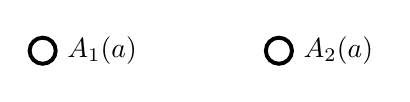
\begin{tikzpicture}
 \node[mynode, label=right:$A_1(a)$] (a1a) at (0, 0) {};
 \node[mynode, label=right:$A_2(a)$] (a2a) at (3, 0) {};
\end{tikzpicture}
\caption{The unique  complete materialization graph of $\mathcal{O}_{\text{ex}_1}$}
\label{fig:ex1}
\end{figure}

\clearpage

\begin{example}\label{exp:dllite}
  Given a (DL-Lite) ontology $\mathcal{O}_{\text{ex}_2}$ where the TBox
  contains the following axioms: $A_1\sqsubseteq B$,
  $A_2\sqsubseteq B$; its ABox contains the assertions $A_1(a)$ and
  $A_2(a)$.  We denote the corresponding datalog program of
  $\mathcal{O}_{\text{ex}_2}$ by
  $P_{\text{ex}_2}=\langle R, \textbf{I}\rangle$, where $R$ contains the
  rules that are transformed from the above axioms ($A_1(x) \to B(x)$,
  $A_2(x) \to A_1(x)$); $\textbf{I}$ contains $A_1(a)$ and $A_2(a)$.
  The two complete materialization graphs of $P_{\text{ex}_2}$ are denoted by
  $\mathcal{G}_{\text{ex}_{2a}}$ and $\mathcal{G}_{\text{ex}_{2b}}$
  (see Figure~\ref{fig:ex2}).

  \textcolor{red}{Note that Figure~\ref{fig:ex2not} does not show a
    materialization graph of $P_{\text{ex}_2}$ since the node $B(a)$
    has the two parents $A_1(a)$ and $A_2(a)$. Hence, there should be
    a rule $A_1(a), A_2(a) \to B(a) \in P_{\text{ex}_2}^*$ by the
    definition of materialization graphs.}
\end{example}

\begin{figure}[htbp]
\centering
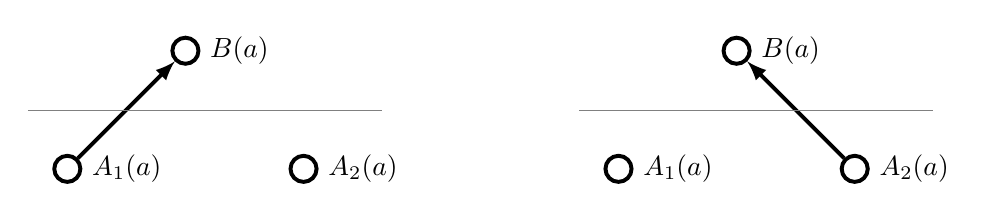
\begin{tikzpicture}
  \begin{scope}
   \node[mynode, label=right:$A_1(a)$] (a1a) at (0, 0) {};
   \node[mynode, label=right:$A_2(a)$] (a2a) at (3, 0) {};
   \node[mynode, label=right:$B(a)$] (ba) at (1.5, 1.5) {};

   \draw[-latex,line width=0.5mm] (a1a) -- (ba);
   \draw[very thin,gray] (-.5, .75) -- (4, .75);
 \end{scope}
  \begin{scope}[xshift=7cm]
   \node[mynode, label=right:$A_1(a)$] (a1a) at (0, 0) {};
   \node[mynode, label=right:$A_2(a)$] (a2a) at (3, 0) {};
   \node[mynode, label=right:$B(a)$] (ba) at (1.5, 1.5) {};

   \draw[-latex,line width=0.5mm] (a2a) -- (ba);
   \draw[very thin,gray] (-.5, .75) -- (4, .75);
 \end{scope}
\end{tikzpicture}
\caption{The complete materialization graphs of $\mathcal{O}_{\text{ex}_2}$}
\label{fig:ex2}
\end{figure}

\begin{figure}[htbp]
\centering
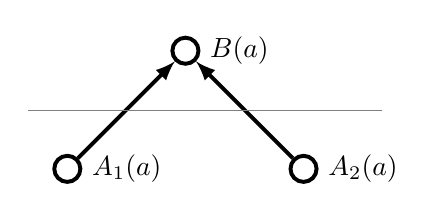
\begin{tikzpicture}
   \node[mynode, label=right:$A_1(a)$] (a1a) at (0, 0) {};
   \node[mynode, label=right:$A_2(a)$] (a2a) at (3, 0) {};
   \node[mynode, label=right:$B(a)$] (ba) at (1.5, 1.5) {};

   \draw[-latex,line width=0.5mm] (a1a) -- (ba);
   \draw[-latex,line width=0.5mm] (a2a) -- (ba);
   \draw[very thin,gray] (-.5, .75) -- (4, .75);
\end{tikzpicture}
\caption{Not a materialization graphs of $\mathcal{O}_{\text{ex}_2}$!}
\label{fig:ex2not}
\end{figure}

\clearpage

\begin{example}\label{exp:dllite}
  Given a (DL-Lite) ontology $\mathcal{O}_{\text{ex}_3}$ where the
  TBox contains the following axiom: $A\sqsubseteq B$; its ABox
  contains the assertions $A(a)$ and $B(a)$.  We denote the
  corresponding datalog program of $\mathcal{O}_{\text{ex}_3}$ by
  $P_{\text{ex}_3}=\langle R, \textbf{I}\rangle$, where $R$ contains
  the rules that are transformed from the above axioms
  ($A(x) \to B(x)$); $\textbf{I}$ contains $A(a)$ and $B(a)$.  The
  unique complete materialization graph of $P_{\text{ex}_3}$ is
  denoted by $\mathcal{G}_{\text{ex}_3}$ (see Figure~\ref{fig:ex3}).

  \textcolor{red}{Note that there cannot be an edge between $A(a)$ and $B(a)$ since
  both are facts and must have in-degree of $0$.}
\end{example}

\begin{figure}[htbp]
\centering
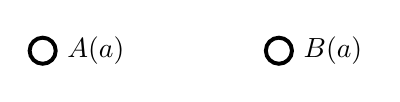
\begin{tikzpicture}
   \node[mynode, label=right:$A(a)$] (aa) at (0, 0) {};
   \node[mynode, label=right:$B(a)$] (ba) at (3, 0) {};
\end{tikzpicture}
\caption{The unique complete materialization graph of $\mathcal{O}_{\text{ex}_3}$}
\label{fig:ex3}
\end{figure}

\clearpage

\begin{example}\label{exp:dllite}
  Given a (DL-Lite) ontology $\mathcal{O}_{\text{ex}_4}$ where the
  TBox contains the following axiom: $A\sqsubseteq B$; its ABox
  contains the assertions $A(a)$ and $B(b)$.  We denote the
  corresponding datalog program of $\mathcal{O}_{\text{ex}_4}$ by
  $P_{\text{ex}_4}=\langle R, \textbf{I}\rangle$, where $R$ contains
  the rules that are transformed from the above axioms
  ($A(x) \to B(x)$); $\textbf{I}$ contains $A(a)$ and $B(b)$.  The
  unique complete materialization graph of $P_{\text{ex}_4}$ is
  denoted by $\mathcal{G}_{\text{ex}_4}$ (see Figure~\ref{fig:ex4}).

  \textcolor{red}{Note that Figure~\ref{fig:ex4incomplete} shows a
    materialization graph of $P_{\text{ex}_4}$, but it is an
    incomplete one since the node $B(a) \not\in V$, but
    $B(a) \in T_R^{\omega}(\textbf{I})$. Figure~\ref{fig:ex4notfacts}
    does not show a materialization graph of $P_{\text{ex}_4}$ since
    $B(b) \not\in V$, but $B(b) \in \textbf{I}$ and
    $\textbf{I} \subseteq V$ is violated. Figure~\ref{fig:ex4not} does
    not show a materialization graph of $P_{\text{ex}_4}$ since the
    node $A(b) \in V \setminus \textbf{I}$ and has no parents. Hence
    there should be $\rightarrow A(b)\in P^*$, which is not the case.}
\end{example}

\begin{figure}[h]
\centering
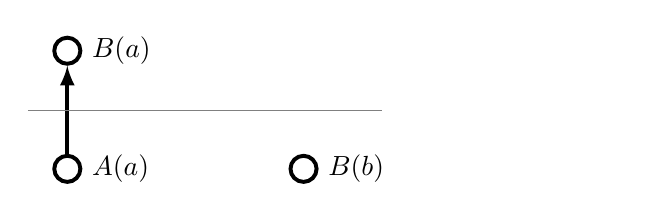
\begin{tikzpicture}
   \node[mynode, label=right:$A(a)$] (aa) at (0, 0) {};
   \node[mynode, label=right:$B(a)$] (ba) at (0, 1.5) {};
   \node[mynode, label=right:$B(b)$] (bb) at (3, 0) {};
   \phantom{\node[mynode, label=right:$A(b)$] (ab) at (6, 0) {};}

   \draw[-latex,line width=0.5mm] (aa) -- (ba);
   \draw[very thin,gray] (-.5, .75) -- (4, .75);
\end{tikzpicture}
\caption{The unique, complete materialization graph of
  $\mathcal{O}_{\text{ex}_4}$ }
\label{fig:ex4}
\end{figure}

\begin{figure}[h]
\centering
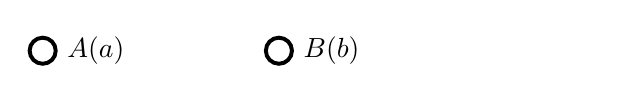
\begin{tikzpicture}
   \node[mynode, label=right:$A(a)$] (aa) at (0, 0) {};
   \node[mynode, label=right:$B(b)$] (bb) at (3, 0) {};
   \phantom{\node[mynode, label=right:$A(b)$] (ab) at (6, 0) {};}
\end{tikzpicture}
\caption{An incomplete materialization graph of
  $\mathcal{O}_{\text{ex}_4}$ }
\label{fig:ex4incomplete}
\end{figure}

\begin{figure}[h]
\centering
\begin{tikzpicture}
   \node[mynode, label=right:$A(a)$] (aa) at (0, 0) {};
   \phantom{\node[mynode, label=right:$A(b)$] (ab) at (6, 0) {};}
\end{tikzpicture}
\caption{Not a materialization graph of
  $\mathcal{O}_{\text{ex}_4}$ due to missing facts}
\label{fig:ex4notfacts}
\end{figure}

\begin{figure}[h]
\centering
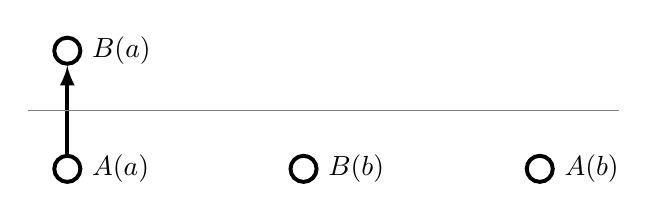
\begin{tikzpicture}
   \node[mynode, label=right:$A(a)$] (aa) at (0, 0) {};
   \node[mynode, label=right:$B(a)$] (ba) at (0, 1.5) {};
   \node[mynode, label=right:$B(b)$] (bb) at (3, 0) {};
   \node[mynode, label=right:$A(b)$] (ab) at (6, 0) {};

   \draw[-latex,line width=0.5mm] (aa) -- (ba);
   \draw[very thin,gray] (-.5, .75) -- (7, .75);
\end{tikzpicture}
\caption{Not a materialization graph of $\mathcal{O}_{\text{ex}_4}$}
\label{fig:ex4not}
\end{figure}

\end{document}

%%% Local Variables:
%%% mode: latex
%%% TeX-master: "fig-dllite"
%%% End:


